\documentclass[conference]{IEEEtran}
\IEEEoverridecommandlockouts

% ── Packages ────────────────────────────────────────────────────────────────
\usepackage{cite}
\usepackage{amsmath,amssymb,amsfonts}
\usepackage{algorithmic}
\usepackage{graphicx}
\usepackage{textcomp}
\usepackage{xcolor}
\usepackage{hyperref}
\usepackage{url}
\usepackage{booktabs}
\usepackage{multirow}
\usepackage{array}
\usepackage{listings}
\usepackage{balance}
\usepackage{pgfplots}
\pgfplotsset{compat=1.17}

% ── Listing style ────────────────────────────────────────────────────────────
\lstset{
  basicstyle=\footnotesize\ttfamily,
  breaklines=true,
  frame=single,
  keywordstyle=\color{blue},
  commentstyle=\color{gray},
  stringstyle=\color{red!70!black}
}

\def\BibTeX{{\rm B\kern-.05em{\sc i\kern-.025em b}\kern-.08em
    T\kern-.1667em\lower.7ex\hbox{E}\kern-.125emX}}

% TODO markers: numbers in Section VI (competency questions) and the
% inter-annotator kappa in Section VII-F are computed against a corpus
% snapshot that is being regenerated as of this draft (full-text scraping +
% translator fix landed; historical backfill + second-annotator labeling
% in progress). Do not submit with the placeholder values below still in
% place -- search for "TODO(refresh)" before submission.
\newcommand{\TODOrefresh}[1]{#1}

% ── Document ─────────────────────────────────────────────────────────────────
\begin{document}

\title{Building and Maintaining a Temporal Knowledge Graph\\
for News Streams on China--Romania Relations}

\author{
\IEEEauthorblockN{Andreea-Maria Onaci}
\IEEEauthorblockA{
\textit{Department of Computer Science}\\
\textit{Technical University of Cluj-Napoca}\\
Cluj-Napoca, Romania\\
andreea.onaci@campus.utcluj.ro
}
\and
\IEEEauthorblockN{Mihaela Macarie-Ancău}
\IEEEauthorblockA{
\textit{Department of Computer Science}\\
\textit{Technical University of Cluj-Napoca}\\
Cluj-Napoca, Romania\\
mihaela.macarie@campus.utcluj.ro
}
\and
\IEEEauthorblockN{Petruț-Betuel Paul}
\IEEEauthorblockA{
\textit{Department of Computer Science}\\
\textit{Technical University of Cluj-Napoca}\\
Cluj-Napoca, Romania\\
petrut.paul@campus.utcluj.ro
}
}

\maketitle

% ── Abstract ─────────────────────────────────────────────────────────────────
\begin{abstract}
We present a system for building and maintaining a temporal knowledge graph
(TKG) from a multilingual news stream restricted to articles that mention
both China and Romania. The pipeline ingests full article text from GDELT
and curated RSS feeds, performs entity and relation extraction via spaCy
and DeepKE, anchors temporal expressions to ISO~8601 intervals using
HeidelTime~TIMEX3 normalization, and stores the resulting graph in Neo4j.
A bilateral-relations ontology grounded in CAMEO/GDELT event codes, IPTC
Media Topics, and W3C OWL-Time governs the semantic structure of events and
their validity intervals, with temporal relations between events computed
under the full 13-relation Allen Interval Algebra rather than a coarse
before/after/overlaps view. A credibility layer combines source-domain
scoring with publisher-network-aware cross-source corroboration,
embedding-based semantic claim merging, and NLI-based contradiction
detection; a temporal gate grounded in the Allen relations, together with an
explicit per-event-type claim-lifecycle state machine, distinguishes
genuine factual contradiction from ordinary claim evolution (e.g.\
\emph{proposed} $\rightarrow$ \emph{signed} $\rightarrow$ \emph{ratified})
before a claim is flagged as contested. Five competency questions drive the
evaluation: tracking economic evolution, surfacing institutional linkages,
enumerating bilateral events, identifying low-credibility narratives, and
discovering collaborative research. We additionally report a rule-based
reproduction of a coarse time-bucket temporal representation from prior
fact-checking work as an ablation baseline for the Allen-relation gate.
Modular architecture and reproducible schema migrations allow incremental
update as new articles arrive, making the system suitable for ongoing
monitoring of a bilateral news domain.
\end{abstract}

\begin{IEEEkeywords}
temporal knowledge graph, news stream processing, bilateral relations,
China--Romania, DeepKE, HeidelTime, TIMEX3, Neo4j, fake-news detection,
GDELT, ontology reasoning, Allen interval algebra, natural language
inference, claim-lifecycle verification
\end{IEEEkeywords}

% ─────────────────────────────────────────────────────────────────────────────
\section{Introduction}
\label{sec:intro}

The diplomatic, economic, and cultural relationship between China and Romania
has intensified significantly since Romania's accession to the European
Union and China's Belt and Road Initiative expanded westward into Central and
Eastern Europe. However, this bilateral domain is served by a heterogeneous,
multilingual news ecosystem whose signals range from state-aligned outlets
(CGTN, Xinhua) to independent Romanian business press and international
wire services. Tracking the evolution of this relationship requires more
than keyword monitoring; it demands structured, time-aware representation
of events and the provenance of every claim.

Knowledge graphs (KGs) have become a standard representation for structured
world knowledge, and temporal knowledge graphs (TKGs)~\cite{trivedi2019dyrep}
extend KGs with valid-time intervals so that facts can be queried relative
to a point in time. Despite an extensive body of work on general-purpose
TKGs (Wikidata, YAGO, EventKG~\cite{gottschalk2019eventkg}), there is no
existing resource dedicated to the China--Romania bilateral domain, and
general-purpose TKGs stop at storing a validity interval per fact: they do
not reason about \emph{how} two intervals relate beyond simple overlap, and
they do not distinguish a claim that genuinely contradicts an earlier one
from a claim that merely reports the next stage of the same real-world
process.

This paper makes the following contributions:
\begin{itemize}
  \item A modular, open-source pipeline that ingests full article text
        (not just headlines), deduplicates, and filters multilingual news
        articles, retaining only those co-mentioning China and Romania.
  \item A bilateral-relations ontology combining CAMEO/GDELT event codes,
        IPTC Media Topics, and W3C OWL-Time for temporal validity, with
        pairwise event relations computed under the complete 13-relation
        Allen Interval Algebra~\cite{allen1983interval}.
  \item Integration of HeidelTime~TIMEX3 normalization and DeepKE for
        joint temporal and relational extraction.
  \item A credibility module that combines publisher-network-aware
        cross-source corroboration, sentence-embedding semantic claim
        merging, and NLI-based contradiction detection, gated by the
        Allen relations and an explicit claim-lifecycle state machine so
        that sequential reporting on an evolving story (e.g.\ a trade deal
        moving from \emph{proposed} to \emph{signed}) is not mistaken for
        a factual contradiction.
  \item A rule-based, same-mechanism-class reproduction of the coarse
        time-bucket temporal representation used in prior evidence-based
        fact-checking work~\cite{allein2023implicit}, used as an ablation
        baseline to justify the added complexity of exact interval-algebra
        reasoning over a bucketed-distance heuristic.
  \item Five competency questions evaluated against the resulting graph.
\end{itemize}

The remainder of this paper is organized as follows. Section~\ref{sec:related} reviews related work, followed by an overview of the high-level system architecture in Section~\ref{sec:architecture}. Sections~\ref{sec:ingestion} and \ref{sec:extraction} detail the data ingestion and information extraction pipelines, respectively. Section~\ref{sec:ontology} presents the bilateral-relations ontology and its Allen-algebra temporal reasoning layer, which informs the graph schema and population discussed in Section~\ref{sec:graph}. Section~\ref{sec:credibility} introduces the credibility assessment layer, including semantic corroboration, NLI contradiction detection, and claim-lifecycle verification. Section~\ref{sec:evaluation} evaluates the system using targeted competency questions and component-level ablations, and Section~\ref{sec:conclusion} concludes the work.

% ─────────────────────────────────────────────────────────────────────────────
\section{Related Work}
\label{sec:related}

\subsection{Temporal Knowledge Graphs}

Temporal KGs extend the standard subject--predicate--object triple with a
validity interval, enabling time-scoped queries. Representative works
include T-REx~\cite{elsahar2018trex}, TimePlex~\cite{jain2020timeplex},
and Know\-Evolution~\cite{trivedi2019dyrep}. EventKG~\cite{gottschalk2019eventkg}
is the closest general-purpose reference for our work, aggregating events
from Wikidata, DBpedia, and YAGO with linked temporal metadata.
None of these resources targets a bilateral news-stream context, incorporates
a live credibility assessment layer, or reasons about interval relations
beyond storing a validity range per fact. Qualitative reasoning about how
two intervals relate to each other is a much older, separate line of work,
formalized by Allen's Interval Algebra~\cite{allen1983interval}: 13
mutually exclusive, jointly exhaustive relations (\emph{before}, \emph{meets},
\emph{overlaps}, \emph{during}, \emph{starts}, \emph{finishes}, \emph{equals},
and their inverses) between two closed intervals. We adopt this formalism
directly for event-pair reasoning in our graph (Section~\ref{sec:ontology})
rather than an ad hoc coarse bucketing of relations, and use it as the
temporal gate that separates genuine contradiction from claim evolution in
the credibility layer (Section~\ref{sec:credibility}).

\subsection{News-Driven Knowledge Graph Population}

The Global Database of Events, Language and Tone
(GDELT)~\cite{leetaru2013gdelt} extracts structured event records from
global news at large scale using the CAMEO event taxonomy~\cite{gerner2002cameo}.
GDELT provides rich provenance metadata but lacks fine-grained temporal
normalization and bilateral-domain ontological grounding; its Full-Text
Search API in particular returns only a title and, in practice, rarely a
usable summary snippet, so a naive integration risks operating on headline
text alone (Section~\ref{sec:ingestion}).

NewsKG and similar systems~\cite{fader2011reverb} populate KGs from news
corpora but do not maintain temporal intervals or include credibility scoring.
Our system builds upon GDELT as an article-discovery backend while adding
full-text extraction, ontology-aligned extraction, and provenance-aware
credibility reasoning.

\subsection{Information Extraction Tools}

DeepKE~\cite{zhang2022deepke} provides unified deep-learning models for
named-entity recognition (NER), relation extraction, and event extraction.
HeidelTime~\cite{strotgen2010heideltime} extracts and normalizes temporal
expressions to the TIMEX3 standard~\cite{pustejovsky2003timex3}, which is
critical for grounding event validity. We combine both tools with a
rule-augmented spaCy pipeline to maximize recall on China--Romania
domain-specific entities, and with trafilatura~\cite{barbaresi2021trafilatura}
for boilerplate-free full-text extraction from raw article HTML.

\subsection{Fake-News, Contradiction, and Credibility Assessment}

Automated credibility assessment of news claims is an active area of
research~\cite{shu2019fakenews}. Approaches range from source-domain
reputation scoring to graph-consistency checks~\cite{popat2018credeyecontrib}
and cross-document corroboration. A related but distinct line of work
studies \emph{implicit temporal reasoning} for fact-checking: Allein
\textit{et al.}~\cite{allein2023implicit} learn a time-bucket embedding per
distance-in-days quantile between an evidence document and a claim and feed
it as a feature to a neural verification model, rather than computing an
exact qualitative relation between the two. Our credibility module integrates
source-domain scoring, publisher-network-aware corroboration, and
cross-document contradiction detection in a lightweight layer that does not
require external fact-checking APIs at inference time, and Section~\ref{sec:evaluation}
reports a direct ablation of exact Allen-relation gating against a rule-based,
same-mechanism-class reproduction of Allein \textit{et al.}'s coarse
time-bucket representation.

Contradiction detection between claim sentences is framed here as a natural
language inference (NLI) problem, using a pretrained cross-encoder built on
DeBERTaV3~\cite{he2021debertav3}; semantic corroboration matching uses
mean-pooled sentence embeddings from a MiniLM-based sentence encoder~\cite{wang2020minilm}.

% ─────────────────────────────────────────────────────────────────────────────
\section{System Architecture}
\label{sec:architecture}

Figure~\ref{fig:architecture} provides a high-level view of the pipeline.
The system is organized into six modules:
\begin{itemize}
    \item Ingestion
    \item Extraction
    \item Temporal Anchoring
    \item Ontology Annotation
    \item Graph Population
    \item Credibility Assessment
\end{itemize}

Intermediate results are persisted in
SQLite (for articles and NLP outputs) before being loaded into Neo4j (for
graph queries). All configuration resides in a single YAML file overlaid by
environment variables, enabling secret-free reproducibility.

\begin{figure*}[htbp]
  \centering
  \includegraphics[width=\textwidth]{top_level_pipeline.eps}
  \caption{Top-level orchestration and data flow of the Temporal KG pipeline.}
  \label{fig:architecture}
\end{figure*}

The pipeline is designed for incremental operation: each module can be
rerun independently, new articles are deduplicated before processing, and
numbered SQL migrations make the SQLite schema reproducible across
deployments.

\section{Ingestion and Relevance Filtering}
\label{sec:ingestion}

\subsection{Article Sources}

The system monitors two complementary article streams:

\paragraph{GDELT Full-Text Search API}
The primary source is the GDELT~2.0 Full-Text Search
API~\cite{leetaru2013gdelt} queried with the term pair
\texttt{"China"~AND~"Romania"}. GDELT returns up to 250 article stubs per
request, each containing a URL, title, and publication timestamp; in
practice the API almost never populates a usable summary snippet for these
stubs. GDELT provides the default credibility score of~0.7 assigned to each
article prior to domain-level adjustment.

\paragraph{Curated RSS Feeds}
Supplementary feeds are polled at configurable intervals (Table~\ref{tab:feeds}).
Feed-level metadata includes a source-country tag and a prior credibility
score used by the credibility module.

\begin{table}[htbp]
\caption{RSS Feeds Monitored by the Ingestion Module}
\label{tab:feeds}
\centering
\small
\begin{tabular}{lll}
\toprule
\textbf{Feed} & \textbf{Focus} & \textbf{Credibility Prior} \\
\midrule
Google News (bilateral) & General & 0.60 \\
Radio Romania International & Political/cultural & 0.80 \\
Bursa.ro (capital markets) & Financial & 0.60 \\
Radio Free Europe & Political & 0.80 \\
\bottomrule
\end{tabular}
\end{table}

\subsection{Pipeline Steps}

Each article stub passes through a nine-step pipeline before persisting to
SQLite. A revision from an earlier version of this pipeline is worth
stating explicitly, since it materially changes what every downstream
module operates on: article text is now \emph{fetched}, not assembled from
title and snippet alone.

\begin{enumerate}
  \item \textbf{URL deduplication}: SHA-256 hash of the URL is checked
        against the seen-URLs table; duplicates are skipped immediately.
  \item \textbf{Full-text scraping}: the article URL is downloaded and its
        main body text is extracted with trafilatura~\cite{barbaresi2021trafilatura}
        (boilerplate removal: navigation, related-links, and comment
        sections are stripped). This step is best-effort: dead links,
        paywalls, and transient failures fall back to title text rather
        than dropping the article, and every failure mode is logged
        rather than silently degrading. GDELT's Full-Text Search API
        returns only a title and (in practice) no usable snippet, so
        without this step the ``article text'' available to every
        downstream module -- NER, relation extraction, temporal
        extraction, and corroboration -- is just the headline. We verified
        this was in fact happening on the full ingested corpus prior to
        this fix (Section~\ref{sec:discussion}).
  \item \textbf{Text assembly}: title and scraped body text (or, on scrape
        failure, title and any GDELT-provided snippet) are concatenated
        into \texttt{content\_clean}.
  \item \textbf{Language detection}: Detected using the \texttt{langdetect}
        library; language tag stored with the article.
  \item \textbf{Translation}: Non-English articles are translated to
        English via a Google-Translate-backed client
        (\texttt{deep-translator}), chunked to the endpoint's per-request
        character limit, with a fixed inter-request delay and a defensive
        check against the endpoint returning an HTML error page as if it
        were a translation (Section~\ref{sec:discussion}), preserving the
        original text in \texttt{content\_raw}.
  \item \textbf{Content hashing}: SHA-256 of the normalized text enables
        a second, content-level deduplication pass.
  \item \textbf{Relevance filtering}: The article must contain at least
        one token from the China alias set and at least one from the Romania
        alias set; irrelevant articles are discarded. A narrow secondary
        exclusion additionally drops otherwise-relevant articles that trip a
        sports-competition marker (competition-governing-body acronyms and
        explicit sports-section tags). This was added after full-text
        scraping surfaced a real failure mode: a genuine China-vs-Romania
        table-tennis match report satisfies plain co-occurrence, but sports
        results are out of scope for this project's 11-type bilateral
        \emph{relations} ontology, and a multi-match roundup article can leak
        an unrelated match's sentence into event extraction. On the current
        corpus, this excluded 8 of 112 previously-relevant articles (three
        table-tennis reports, a judo report, and coverage of the World
        Aquatics Championships), and eliminated one of the corpus's 17
        contradictory claim groups that traced directly to this failure mode.
  \item \textbf{Persistence}: Relevant articles are written to SQLite
        and optionally exported as JSON.
  \item \textbf{Deduplication registration}: URL and content hashes are
        registered in memory for future deduplication within the same run.
\end{enumerate}

This two-stage deduplication (URL hash first, content hash second) reduces
redundancy from syndicated content while preserving the same story covered
by independent outlets, which is important for corroboration. It is,
however, not sufficient on its own to make cross-outlet corroboration
counts meaningful, since many outlets mirror the exact same wire-service
copy rather than independently reporting it; Section~\ref{sec:credibility}
describes how the credibility layer corrects for this.

% ─────────────────────────────────────────────────────────────────────────────
\section{Entity, Relation, and Temporal Extraction}
\label{sec:extraction}

\subsection{Named Entity Recognition}

Entity extraction follows a \emph{rule-first, model-augmented} strategy.
The rule layer handles domain-specific surface forms with high precision,
while the model layer provides recall on unseen names.

\paragraph{Rule-based extraction}
Four deterministic passes operate on each sentence:
\begin{itemize}
  \item \textbf{Country mentions}: alias tables for ``China'' (PRC,
        Chinese, People's Republic of China) and ``Romania'' (\textit{România},
        Romanian) with regex boundary matching.
  \item \textbf{Location mentions}: a curated gazetteer covering major
        Chinese and Romanian cities (Beijing, Bucharest, Shanghai, Cluj-Napoca,
        Constanța, etc.).
  \item \textbf{Person mentions}: capitalized multi-word tokens following
        a title keyword (President, Prime Minister, Ambassador, Ministrul,
        Ambasadorul).
  \item \textbf{Organization mentions}: capitalized spans containing
        organizational keywords (Ministry, Embassy, University, Bank,
        Council) or abbreviation patterns.
\end{itemize}
Each mention is assigned a confidence score: 1.0 for country tokens,
0.93 for title-anchored persons, 0.90 for keyword-matched organizations,
and 0.74 for heuristic capitalized-span persons.

\paragraph{DeepKE integration}
When DeepKE~\cite{zhang2022deepke} is enabled, the system invokes a
configured command template, writes a per-article JSON input, and reads the
structured output. DeepKE mentions are merged with rule-based mentions using
a span-deduplication key \texttt{(start\_char, end\_char, entity\_type)}.

\paragraph{spaCy model augmentation}
If a spaCy language model is available (\texttt{en\_core\_web\_sm} by
default), it provides sentence boundaries and can be extended with
domain-adapted NER components.

\subsection{Relation Extraction}

Relation extraction maps entity pairs within a sentence to predicate types
drawn from the bilateral ontology (Section~\ref{sec:ontology}). Pattern-based
rules cover the most frequent surface realizations (e.g., \textit{``X
signed an agreement with Y''}, \textit{``X invested in Y''}); DeepKE's
relation-extraction module supplements these with learned patterns.

\subsection{Temporal Expression Extraction}

Temporal extraction relies on HeidelTime~\cite{strotgen2010heideltime} via
the \texttt{py-heideltime} Python package. HeidelTime annotates text with
TIMEX3 tags and normalizes them to ISO~8601. Table~\ref{tab:timex} shows
the TIMEX3 types handled.

\begin{table}[htbp]
\caption{TIMEX3 Expression Types Handled by HeidelTime}
\label{tab:timex}
\centering
\small
\begin{tabular}{lll}
\toprule
\textbf{Type} & \textbf{Example} & \textbf{ISO Normalized} \\
\midrule
DATE     & ``12 May 2026''         & \texttt{2026-05-12} \\
DATE     & ``last week''           & \texttt{2026-W22} \\
DURATION & ``for three months''    & \texttt{P3M} \\
SET      & ``every year''          & \texttt{XXXX} \\
TIME     & ``at 14:00''            & \texttt{T14:00} \\
INTERVAL & ``valid until 2030''    & \texttt{2026-05/2030} \\
\bottomrule
\end{tabular}
\end{table}

When \texttt{py-heideltime} is unavailable (e.g., Java or Perl not
installed), the system falls back to a hand-crafted regex engine covering
the most common absolute date patterns. Extracted temporal expressions are
linked to event nodes in the graph as \texttt{validFrom}/\texttt{validTo}
interval endpoints, following W3C OWL-Time semantics, and feed directly into
the Allen-relation reasoning described in Section~\ref{sec:temporal-reasoning}.

\begin{figure}[htbp]
  \centering
  \includegraphics[width=\linewidth]{combined_extraction_sequence.eps}
  \caption{Sequence diagram of the combined extraction module.}
  \label{fig:extraction}
\end{figure}

\section{Bilateral-Relations Ontology}
\label{sec:ontology}

\subsection{Event Taxonomy}

The ontology defines 11 bilateral event types grounded in three established
classifications (Table~\ref{tab:taxonomy}).

\begin{table*}[htbp]
\caption{Bilateral Event Taxonomy with CAMEO, GDELT, and IPTC Mappings}
\label{tab:taxonomy}
\centering
\small
\begin{tabular}{p{3.2cm}p{3.0cm}p{3.2cm}p{4.2cm}}
\toprule
\textbf{Event Type} & \textbf{CAMEO Code} & \textbf{GDELT Category}
  & \textbf{IPTC Topic} \\
\midrule
DiplomaticMeeting      & 04 Consult                           & Diplomatic Cooperation    & Politics/Diplomacy \\
TradeAgreement         & 07 Provide Aid                       & Economic Cooperation      & Economy/Trade \\
InvestmentProject      & 08 Yield                             & Economic Investment       & Economy/Investment \\
TechnologyCooperation  & 05 Diplomatic Cooperation            & Science and Technology    & Science/Research \\
InfrastructureProject  & 07 Provide Aid                       & Infrastructure            & Economy/Construction \\
EducationCooperation   & 05 Diplomatic Cooperation            & Education                 & Education \\
SecurityStatement      & 13 Threaten                          & Security                  & Crime/Defence \\
SanctionOrRestriction  & 11 Sanctions                         & Sanctions                 & Politics/Sanctions \\
CompanyActivity        & 07 Provide Aid                       & Corporate Activity        & Economy/Companies \\
CulturalExchange       & 05 Diplomatic Cooperation            & Cultural Exchange         & Arts/Culture \\
PolicyStatement        & 01 Public Statement                  & Policy                    & Politics \\
\bottomrule
\end{tabular}
\end{table*}

\subsection{Temporal Validity Model}

Each event node carries:
\begin{itemize}
  \item \texttt{validFrom} -- earliest ISO~8601 date extracted from the
        reporting article or TIMEX3 tag.
  \item \texttt{validTo} -- latest bound, or \texttt{null} for open-ended
        intervals.
  \item \texttt{temporalGranularity} -- one of \{day, month, year\}.
\end{itemize}
This models the W3C OWL-Time Interval and Instant classes~\cite{cox2017owltime}
and aligns with the EventKG temporal representation~\cite{gottschalk2019eventkg}.

\subsection{Allen-Relation Reasoning Between Events}
\label{sec:temporal-reasoning}

Storing a validity interval per event is necessary but not sufficient for
answering questions like \emph{``did these two reports describe the same
occurrence, or two different stages of an evolving story?''} We compute the
exact qualitative relation between every pair of event intervals under
Allen's Interval Algebra~\cite{allen1983interval}: 13 mutually exclusive,
jointly exhaustive relations (\emph{before}, \emph{after}, \emph{meets},
\emph{met\_by}, \emph{overlaps}, \emph{overlapped\_by}, \emph{starts},
\emph{started\_by}, \emph{during}, \emph{contains}, \emph{finishes},
\emph{finished\_by}, \emph{equals}) between two closed intervals
$A=[s_1,e_1]$ and $B=[s_2,e_2]$. A point-in-time event (a single reported
date, the common case in news reporting) is represented as a degenerate
interval with $s=e$.

An earlier version of this module collapsed the algebra into five coarse
buckets (\emph{before}/\emph{after}/\emph{contains}/\emph{during}/\emph{overlaps}),
silently merging \emph{meets} (two intervals that share exactly one
boundary point) into \emph{before}, and \emph{equals} into \emph{overlaps}.
This under-serves a temporal-KG reasoning claim: two same-day reports of an
event and two reports of genuinely overlapping-but-distinct events are a
materially different relationship, and conflating them discards information
a downstream consumer -- including the credibility layer's temporal gate,
Section~\ref{sec:credibility} -- would need. The full 13-relation algebra is
now computed directly (\texttt{src/temporal/reasoner.py}); the original
5-bucket view remains available via an explicit coarsening function for
call sites that only need it. A single ambiguity in the algebra's boundary
cases is resolved deterministically: a point event whose date coincides
with another interval's start simultaneously satisfies both \emph{meets}
and \emph{starts}; our implementation checks full equality first (two
point events on the same date are \emph{equals}, not \emph{meets}), then
touching-boundary relations, then same-start/same-end relations, so the
relation returned is always the most specific one that actually holds.

\subsection{Provenance Model}

Every event is linked to its source articles via \texttt{:REPORTED\_BY}
edges carrying the source URL, publication timestamp, and credibility score.
This enables provenance-aware queries such as \emph{``Which articles
reported on this trade agreement?''} and supports the credibility module's
cross-source corroboration check.

% ─────────────────────────────────────────────────────────────────────────────
\section{Graph Schema and Population}
\label{sec:graph}

\subsection{Neo4j Schema}

The graph is stored in Neo4j~4.x with the schema shown in
Figure~\ref{fig:schema}. The main node labels are:

\begin{itemize}
  \item \textbf{Entity} (supertypes: Person, Organization, Location, Country)
  \item \textbf{Event} (sub-typed by the 11 ontology classes)
  \item \textbf{Article} (source document with provenance metadata)
  \item \textbf{TemporalExpression} (TIMEX3-normalized date or interval)
\end{itemize}

Key relationship types include \texttt{PARTICIPATED\_IN}, \texttt{OCCURRED\_AT},
\texttt{VALID\_DURING}, \texttt{REPORTED\_BY}, and \texttt{CORROBORATES}.


  \begin{figure}[htbp]
      \centering
      \includegraphics[width=\linewidth]{property_graph_schema.png}
      \caption{Neo4j graph schema for the China--Romania temporal KG.}
      \label{fig:schema}
  \end{figure}

\subsection{Graph Loading}

The \texttt{GraphLoader} class translates SQLite rows (articles, entities,
events, temporal expressions) into batched Cypher \texttt{MERGE} statements.
The MERGE pattern prevents duplicate nodes across incremental runs. Indexes
on \texttt{Entity.canonical\_name}, \texttt{Event.event\_type}, and
\texttt{Article.url\_hash} ensure query performance. Neo4j itself is
deployed via a single Docker container (\texttt{neo4j:4.4}, credentials
supplied via \texttt{config/.env}, gitignored), requiring no host-level
installation. The full initialization procedure is:

\begin{lstlisting}[language=bash, caption={Graph initialization and population commands.}]
# Start Neo4j (Docker; no host install needed)
docker run -d --name temporal-kg-neo4j \
  -p 7474:7474 -p 7687:7687 \
  -e NEO4J_AUTH=neo4j/<password> \
  -v ~/neo4j_data:/data neo4j:4.4

# Initialise schema (constraints + indexes)
python scripts/init_graph_schema.py

# Populate from SQLite
python scripts/load_graph.py

# Verify population
python scripts/check_neo4j.py
\end{lstlisting}

% ─────────────────────────────────────────────────────────────────────────────
\section{Credibility Assessment Layer}
\label{sec:credibility}

\subsection{Source-Domain Scoring}

Each article is assigned a credibility score by \texttt{CredibilityScorer},
which maps domain names to empirically derived trust levels. State-controlled
outlets receive lower base scores; established independent press receives
higher scores. Per-feed priors (Table~\ref{tab:feeds}) are further adjusted
by:
\begin{itemize}
  \item Presence of named author ($+$0.05)
  \item Publication in the last 24 hours ($+$0.03)
  \item Number of hyperlinks in text (proxy for sourcing)
\end{itemize}

\subsection{Publisher-Network-Aware Source Diversity}
\label{sec:publisher-networks}

A naive corroboration count treats every distinct domain as an independent
source. This overcounts corroboration for large state media operations that
republish the same wire copy across many language-specific domains: a single
Xinhua/People's Daily story about a bilateral diplomatic visit was observed,
on real ingested data, to appear under eight distinct domains
(\texttt{arabic.news.cn}, \texttt{french.xinhuanet.com},
\texttt{spanish.peopledaily.com.cn}, and five others) -- eight regional
mirrors of two institutions, not eight independently reporting outlets.
We resolve each source domain to a shared publisher-network identifier via a
configured domain-suffix mapping before computing \texttt{source\_diversity},
so that this case counts as diversity~2 (Xinhua, People's Daily), not~8.
Domains that do not match a configured network resolve to themselves, so
this mapping only ever reduces an inflated diversity count for known
multi-domain operations -- it never fabricates diversity elsewhere.
On the current (RSS-sourced) corpus, this correction changed
\texttt{source\_diversity} for 2 of 898 claim groups -- a small share
overall, since 95\% of groups in this corpus are single-source and have no
raw-domain overcount to correct in the first place, but the effect on the
groups where it does apply is large: the flagship example above drops from
8 raw domains to 5 independent publisher networks. The mapping is expected
to affect a larger share of groups once the historical GDELT-sourced
backfill (Section~\ref{sec:discussion}) restores higher-redundancy,
wire-service-heavy coverage.

\subsection{Semantic Corroboration Merging}

Claim groups were previously formed only by an \emph{exact} signature match
(event type, participants, and date, or the fully normalized claim
sentence), which misses the common case of two independent outlets covering
the same event in different words (e.g.\ ``Romania and China signed an
energy deal'' vs.\ ``Bucharest and Beijing finalized an agreement on energy
cooperation''). We add a second matching layer: claim sentences are embedded
with a mean-pooled MiniLM sentence encoder~\cite{wang2020minilm}, and
same-event-type groups whose representative sentences exceed a cosine-similarity
threshold ($\tau{=}0.75$) are merged via union-find into a single
corroboration group before support-count, source-diversity, and contradiction
statistics are computed.

\subsection{NLI-Based Contradiction Detection}

A purely structural contradiction flag -- firing only when a corroboration
group contains members with more than one event type or more than one date
window -- is blind to the case that matters most for credibility assessment:
two articles can land in the same group (same event type, same date, correctly
merged as ``about the same event'') while asserting incompatible facts within
it (``12 people were injured'' vs.\ ``2 people were injured''; ``the deal was
signed'' vs.\ ``the deal collapsed''). We run a pretrained natural language
inference (NLI) cross-encoder (\texttt{cross-encoder/nli-deberta-v3-xsmall},
built on DeBERTaV3~\cite{he2021debertav3}) over pairs of distinct claim
sentences within a group, checked in both premise/hypothesis directions
(NLI is directional; which report is treated as the premise between two
independently published claims is arbitrary), and take the maximum
contradiction probability across both orderings. A cheap embedding-similarity
pre-filter (using the same MiniLM encoder as Section~\ref{sec:publisher-networks})
gates the NLI call: NLI models trained on MNLI-style data code many
off-topic pairs as ``contradiction'' rather than the ``neutral'' a human
annotator would assign, so pairs below a relevance-similarity floor
($\tau{=}0.15$) are skipped before the NLI call.

\subsection{Temporal Gating: Contradiction vs.\ Claim Evolution}

Not every NLI-flagged disagreement is a real contradiction. Two reports
disagreeing about ``the deal was proposed'' vs.\ ``the deal was signed''
are not contradicting each other if their extracted event dates occupy
different, non-coincident points in the claim's lifecycle -- they are
describing sequential stages of the same real-world process. We use the
exact Allen relation (Section~\ref{sec:temporal-reasoning}) between the two
claims' date ranges to distinguish the two cases: an NLI disagreement
between claims whose dates stand in a \emph{before}, \emph{after},
\emph{meets}, or \emph{met\_by} relation is reclassified as \emph{claim
evolution} rather than contradiction, since the two reports do not describe
the same instant. Every other relation (\emph{equals}, \emph{overlaps},
\emph{during}, \emph{contains}, \emph{starts}, \emph{finishes}, and their
inverses) means the two claims' time windows genuinely coincide, so an NLI
disagreement between them is treated as a real contradiction. When either
date is unresolved, there is no temporal evidence to justify reclassification,
so the disagreement is conservatively kept as a contradiction.

\subsection{Claim-Lifecycle State Verification}
\label{sec:lifecycle}

The pairwise temporal gate above is still limited in two ways: it considers
only one pair of claims at a time, never a full multi-claim sequence, and it
accepts \emph{any} sequential-dates disagreement as legitimate evolution,
even when the resulting sequence of states does not correspond to a
plausible real-world process (e.g.\ a report of ``ratified'' chronologically
\emph{preceding} a report of ``signed'' looks identical to the pairwise gate
-- sequential dates plus NLI disagreement -- as a genuine inconsistency does).

We address this with an explicit finite-state lifecycle model per event
type (Table~\ref{tab:lifecycles}): a small set of named states (3--5 per
type) and a legal-transition graph between them, hand-authored as a
first-pass domain ontology rather than validated against diplomatic- or
economic-process literature. A claim sentence is mapped to its
best-matching lifecycle state by zero-shot classification: the entailment
probability, under the same NLI cross-encoder used for contradiction
detection above, between the claim sentence (as premise) and a fixed
natural-language template per candidate state (as hypothesis) is computed
for every state in the event type's lifecycle, and
the highest-scoring state above a confidence threshold ($0.5$) is selected
(unclassified otherwise). Given a group of claims flagged as candidate claim
evolution, we date-sort every classified claim in the group and check the
resulting state sequence against the event type's transition graph:
consecutive states with no legal transition between them are flagged as a
genuine \texttt{lifecycle\_violation}, overriding the pairwise gate's
``evolution'' verdict back to a contradiction; consecutive repeats of the
same state (e.g.\ two independent sources both reporting ``signed'') are
never treated as a violation.

\begin{table}[htbp]
\caption{Example Claim-Lifecycle State Machines}
\label{tab:lifecycles}
\centering
\small
\begin{tabular}{ll}
\toprule
\textbf{Event Type} & \textbf{Legal State Sequence(s)} \\
\midrule
TradeAgreement & proposed $\to$ negotiating $\to$ signed $\to$ ratified \\
               & proposed / negotiating / signed $\to$ rejected \\
InvestmentProject & announced $\to$ under\_construction $\to$ completed \\
                   & (either state) $\to$ suspended $\to$ resumed/completed \\
DiplomaticMeeting & scheduled $\to$ (postponed)$^{*}$ $\to$ held / cancelled \\
SanctionOrRestriction & proposed $\to$ imposed $\to$ extended $\to$ lifted \\
\bottomrule
\end{tabular}
\end{table}

\subsection{Claim Verification Labels}

Combining the structural, semantic-contradiction (temporal-gated and
lifecycle-verified), support-count, and source-diversity signals, claims
are classified into three verification statuses:

\begin{enumerate}
  \item \textbf{Corroborated} -- support\_count $\geq 3$ and
        publisher-network diversity $\geq 2$, with no structural or
        semantic contradiction.
  \item \textbf{Weakly supported} -- support\_count $\geq 2$ but below the
        corroborated threshold, with no contradiction.
  \item \textbf{Contested} -- a structural contradiction (multiple event
        types or date windows in one signature group), or a semantic
        contradiction that survives the temporal gate and lifecycle check.
  \item \textbf{Unresolved} -- everything else (typically support\_count
        $=1$, i.e.\ a single-source claim with no corroborating report yet).
\end{enumerate}

\begin{figure}[htbp]
  \centering
  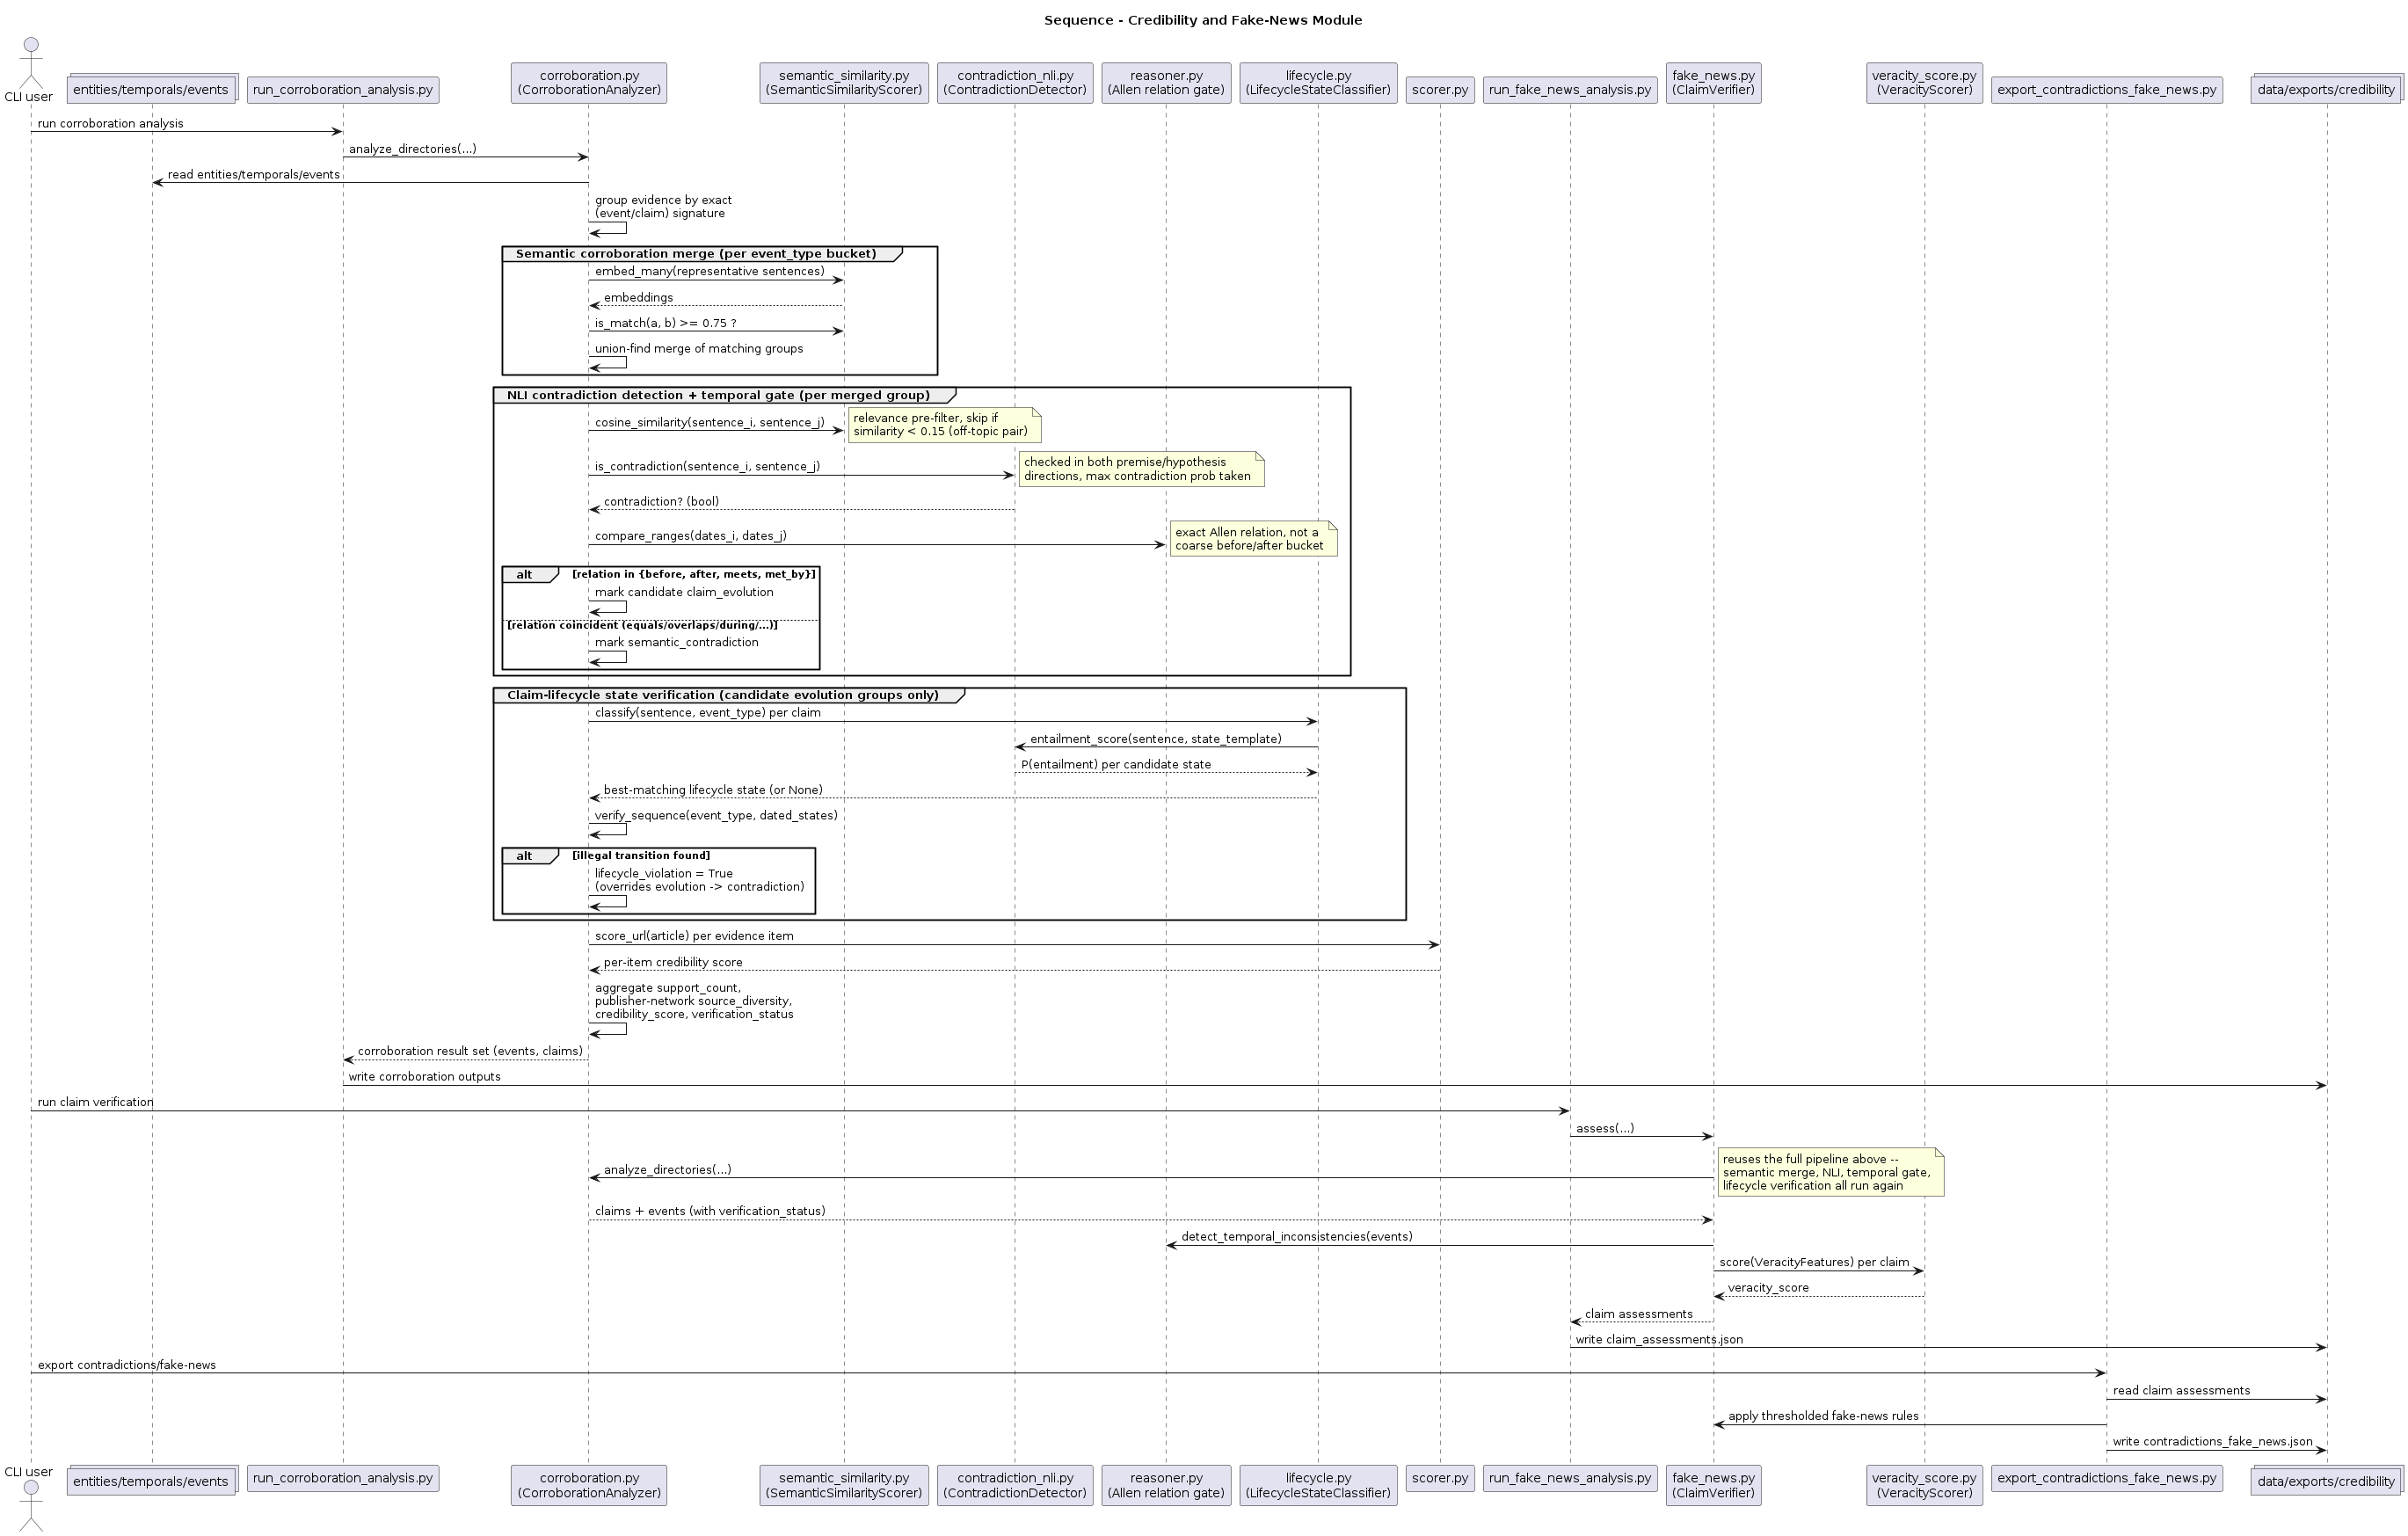
\includegraphics[width=\linewidth]{16_seq_module_credibility.png}
  \caption{Sequence diagram of the credibility assessment module,
  including semantic corroboration merging, NLI contradiction detection
  with its relevance pre-filter, the Allen-relation temporal gate, and
  claim-lifecycle state verification.}
  \label{fig:credibility}
\end{figure}

\section{Evaluation}
\label{sec:evaluation}

\subsection{Component-Level Ablations}
\label{sec:ablations}

Before evaluating the populated graph end-to-end, we validate each new
credibility-layer component in isolation, first against small hand-labeled
gold pair sets (Table~\ref{tab:ablations}), then, for two of the three
components, against much larger real-data pools mined directly from the
corpus (Table~\ref{tab:ablations-scaled}) -- the hand-labeled sets calibrate
default thresholds and validate the core mechanism, the real-data pools
stress-test those thresholds against naturally-occurring text rather than
constructed examples.

\begin{table}[htbp]
\caption{Component Ablations on Hand-Labeled Gold Pairs}
\label{tab:ablations}
\centering
\small
\begin{tabular}{lccc}
\toprule
\textbf{Configuration} & \textbf{P} & \textbf{R} & \textbf{F1} \\
\midrule
\multicolumn{4}{l}{\textit{NLI contradiction detection ($n=10$)}} \\
\quad NLI, $\tau{=}0.5$ & 0.833 & 1.000 & 0.909 \\
\midrule
\multicolumn{4}{l}{\textit{Semantic corroboration matching ($n=10$)}} \\
\quad MiniLM cosine, $\tau{=}0.75$ & 1.000 & 1.000 & 1.000 \\
\midrule
\multicolumn{4}{l}{\textit{Contradiction vs.\ claim evolution ($n=12$)}} \\
\quad Date-mismatch only (no NLI) & 0.143 & 0.200 & 0.167 \\
\quad NLI only (no temporal gate) & 0.500 & 1.000 & 0.667 \\
\quad NLI + coarse time-bucket gate~\cite{allein2023implicit} & 1.000 & 0.800 & 0.889 \\
\quad NLI + exact Allen-relation gate & 1.000 & 1.000 & 1.000 \\
\bottomrule
\end{tabular}
\end{table}

The contradiction-vs.-evolution ablation is the most informative of the
three: a naive date-mismatch-only baseline (flag a contradiction whenever
two dates differ at all, ignoring NLI content entirely) performs barely
above chance (F1~$=0.167$) on this set, confirming that date agreement
alone is not a useful contradiction signal. Adding NLI without any temporal
gate (F1~$=0.667$) recovers all true contradictions but also flags every
same-day claim-evolution pair as contradictory, since NLI has no notion of
time. Gating NLI disagreement by the coarse time-bucket representation from
Allein~\textit{et al.}~\cite{allein2023implicit} -- a same-mechanism-class,
rule-based reproduction of the distance-quantile idea behind their learned
embedding, used here specifically to isolate the representation from their
neural model -- recovers precision (F1~$=0.889$) but misses one contradiction
whose two reports fall in different coarse buckets despite genuinely
overlapping intervals (an \emph{interval\_001} case in our set: the coarse
bucket sees the two dates as ``not close,'' while the exact Allen relation
correctly identifies \emph{contains}). Gating by the exact Allen relation
instead recovers this case and achieves perfect precision and recall on
this set (F1~$=1.000$), which is the empirical justification, within the
limits of a 12-pair set, for reasoning over the full interval algebra
rather than a coarse distance bucket.

\subsection{Ablations on Large Real-Data Pools}
\label{sec:ablations-scaled}

The hand-labeled sets above validate each mechanism but cannot support a
strong empirical claim at $n{=}10$--$12$. For two of the three components we
mined much larger real pools directly from the corpus, using
uncertainty-sampling-style selection (Section~\ref{sec:llm-judge} below):
for semantic matching, all pairwise MiniLM cosine similarities within each
event-type bucket across the corpus's exact-signature claim groups (2{,}132
real comparisons), stratified into the 54 pairs the algorithm actually
predicts as matches, the 50 hardest near-threshold non-matches, and 30 easy
non-matches (134 total); for NLI contradiction, every distinct-sentence pair
within real corroboration groups (334 real comparisons), stratified
similarly (142 total). Two independent cold-started LLM judges (identical
methodology to Section~\ref{sec:llm-judge}) labeled each pool blind; pairs
where both judges agreed form the consensus gold standard.

\begin{table}[htbp]
\caption{Component Ablations on Large Real-Data Pools}
\label{tab:ablations-scaled}
\centering
\small
\begin{tabular}{lcccc}
\toprule
\textbf{Configuration} & $\boldsymbol{n}$ & \textbf{P} & \textbf{R} & \textbf{F1} \\
\midrule
Semantic matching, $\tau{=}0.75$ & 98/134 & 1.000 & 0.690 & 0.817 \\
NLI contradiction, $\tau{=}0.5$ & 141/142 & 0.000 & 0.000 & 0.000 \\
\bottomrule
\end{tabular}
\end{table}
($n$ = consensus-labeled pairs / total mined pairs; judges' Cohen's~$\kappa$
was $0.461$, ``moderate,'' for semantic matching and $0.797$, ``substantial,''
for contradiction.)

\textbf{Semantic matching holds up, conservatively.} At scale, the
$\tau{=}0.75$ threshold has perfect precision (it never merges two
consensus-labeled distinct events) but only $0.690$ recall -- it misses
real duplicate reporting below the threshold. The lower inter-judge
$\kappa$ here (0.461 vs.\ 0.731 for the corroboration-mining task in
Section~\ref{sec:llm-judge}) is itself expected, not a data-quality
problem: that earlier pool drew only from already-merged, mostly
clearly-same-event pairs, while this pool was deliberately stratified
toward the threshold boundary, i.e.\ the genuinely hard cases where two
careful readers can reasonably disagree.

\textbf{NLI contradiction detection does not hold up at scale, and this is
worth stating plainly rather than burying it.} Against the 141-pair
consensus, the raw NLI signal's precision and recall are both
\emph{exactly zero}: of 82 pairs it flags as contradictory, 81 are
false positives, and the 2 genuine contradictions the judges agreed on
(both concerning Huawei's role in Romania's 5G network -- one source
saying it ``played a significant role,'' another that Romania ``rejects
partnering with Huawei'') were not among them. Manual inspection of the
false positives shows a specific, previously-undetected failure mode: the
model is not confusing real content, it is scoring \emph{near-identical
headlines differing only in trailing site attribution} as 99.6\%
contradictory (two reports of the same Belt-and-Road exhibition, one
tagged ``Southern Net,'' one ``Qilu.com''), and scoring
\emph{genuinely different but structurally near-identical diplomatic
press-release sentences} (three separate real Sun Haiyan meetings, on
different dates, with different counterparts -- Adrian Nastase, an IDCPC
Romania delegation visit, and a Bulgarian Socialist Party delegation) at
99.5\%+ as well. The model appears to read ``same sentence template,
different specific facts'' as contradiction rather than the unrelated/
neutral judgment a human gives it, and the cosine-similarity relevance
pre-filter (Section~\ref{sec:credibility}) does not catch this, since these
pairs are genuinely topically similar -- that is precisely what makes them
share a template in the first place. The 10-pair hand-authored set never exposed this because its negative
examples were unrelated sentences, not formulaic near-duplicates; only
real, naturally-occurring press-release text surfaces it. This ablation
isolates the raw NLI signal, the same ``NLI only (no temporal gate)'' row
as Table~\ref{tab:ablations} -- production (Section~\ref{sec:credibility})
additionally applies the Allen-relation temporal gate before finalizing a
contradiction flag, which recovers exactly the cases above where the two
misclassified sentences carry different, non-coincident dates (all three
Sun Haiyan examples do). It does \emph{not} help when an NLI false positive
occurs between same-time-window text, such as the two near-duplicate
Belt-and-Road headlines, since the gate has no temporal evidence to
reclassify a same-day pair. This means the real exposure at the corpus
level is narrower than raw-NLI precision alone would suggest, but is not
zero: some fraction of the corpus's 16 contradictory claim groups
(Section~\ref{sec:cq}) plausibly reflect exactly this same-time-window NLI
misfire rather than genuine content disagreement, and that fraction has not
been individually verified at scale -- a real, now-quantified limitation of
the contradiction-detection layer, not a hypothetical one.

We attempted the same real-data scale-up for the contradiction-vs.-claim-evolution
ablation but could not: only one claim group in the current corpus has more
than one distinct reported date window for the same story, and that one is
off-topic noise, not a genuine China--Romania case. This is a direct
consequence of the corpus's current small scale (Section~\ref{sec:discussion})
rather than a methodological gap -- a larger, GDELT-inclusive corpus with
more repeat/wire coverage of the same evolving stories over time is expected
to make this mineable, and the $n{=}12$ hand-authored set
(Table~\ref{tab:ablations}) remains the only evidence for that component
until then.

\subsection{LLM-Judge Concordance on Real Mined Pairs}
\label{sec:llm-judge}

A second, independent \emph{human} annotator's blind labels over real
(not hand-constructed) candidate pairs mined from the live corpus were
attempted but not obtained for this draft: repeated single-annotator
labeling passes over multi-hundred-pair sets showed timing patterns
(sub-second inter-answer intervals, uniform labels) inconsistent with an
actual per-pair read, even after adding an enforced minimum think-time
between answers to the labeling tool. Rather than omit external validation
entirely or substitute a non-independent judgment, we report a different,
honestly-labeled substitute: \emph{concordance between two independent
LLM judges}. Two separate cold-started agent instances, with no shared
context with each other, with the codebase, or with the semantic-merge
threshold under test, were each given only the raw sentence pairs (stripped
of all source/provenance metadata) and asked the same binary question a
human annotator would answer: do these two sentences describe the same
underlying real-world claim? This is \emph{not} equivalent evidence to
human inter-annotator agreement -- LLM judges carry their own systematic
biases distinct from human ones, and we make no claim that this substitutes
for a genuine human-validated benchmark. We report it as a weaker but real,
honestly disclosed signal, on the same 203 real mined pairs from
Section~\ref{sec:ablations}'s corpus.

The two judges reached Cohen's~$\kappa=0.731$ (``substantial'' agreement
on the Landis \& Koch~\cite{landiskoch1977kappa} scale), 88.7\% observed
agreement across all 203 shared pairs. Two findings from the 23
disagreements are worth reporting on their own: (1)~\emph{every}
disagreement runs the same direction -- judge~A labeled the pair
\emph{same-claim} and judge~B did not, never the reverse -- indicating a
consistent leniency asymmetry between the two judges rather than
symmetric noise; and (2)~disagreements skew toward the semantic-merge
decision boundary: the 23 disputed pairs have median cosine similarity
$0.793$ against a corpus-wide median of $0.803$ (both computed with the
same MiniLM encoder as the merge step itself), a modest but real signal
that ambiguity concentrates near the $\tau=0.75$ threshold rather than
being uniformly distributed -- consistent with treating this as an
uncertainty-sampling problem (selecting pairs for review by proximity to
a decision boundary, the core idea behind active-learning query
strategies such as VisLED-Querying~\cite{ross2024visled}, though that work
targets open-set 3D object detection rather than text-pair verification).

\subsection{Competency Questions}
\label{sec:cq}

We evaluate the structural integrity, expressive capacity, and practical
utility of the populated Temporal Knowledge Graph (TKG) by executing the
five competency questions (CQs) defined during the system requirement
phase~\cite{gruninger1995ontology}, via \texttt{src/graph/competency\_queries.py}'s
Cypher queries against a populated Neo4j~4.4 instance (Docker deployment,
loaded via \texttt{init\_graph\_schema.py} / \texttt{load\_graph.py} as
described in Section~\ref{sec:graph}). The numbers below reflect the
RSS-sourced corpus described in Section~\ref{sec:discussion} -- GDELT's
Full-Text Search API has been unreachable for an extended period at the
time of this draft, so the historical backfill that would substantially
grow this corpus has not yet landed. These are real numbers from a real
graph query, not a placeholder, but they should be read as
corpus-scale-appropriate, not as the system's ceiling.

\subsubsection{Article-Level vs.\ Event-Level Bilateral Gating}
\label{sec:cq-method}

Before the graph was available, we cross-checked query logic by
approximating CQ1--CQ5 directly against the JSON exports, gating on
article-level China+Romania co-occurrence (guaranteed by
\texttt{RelevanceFilter} for every article in the corpus) rather than the
Cypher queries' stricter requirement that China and Romania entities be
direct \texttt{INVOLVES} participants of the \emph{specific event}. The gap
between the two turned out to be large, not a minor rounding difference:
the article-level approximation overcounted CQ1 by $4.0\times$ (355 vs.\
the graph's 88), CQ3 by $3.9\times$ (1{,}146 vs.\ 297), and CQ2 by
$9.3\times$ (28 vs.\ 3). This is itself a real, quantified finding worth
stating: many events' extracted participants (syntactic dependency
arguments of the trigger verb) do not include the literal country-name
entity even when it appears elsewhere in the same article, so
article-level co-occurrence is a substantially looser proxy for
``this event is about China and Romania'' than a true per-event
entity-participant join. All numbers below are the authoritative
graph-native ones. Separately, the raw \texttt{Claim} nodes
\texttt{GraphLoader} populates use exact-signature grouping only -- they do
not carry the semantic-merge / NLI-contradiction / temporal-gate /
lifecycle-verification enrichment from Section~\ref{sec:credibility},
which exists only in \texttt{corroboration.claims.json}. CQ4 therefore
draws from that enriched output, not the raw graph, since it is where this
paper's actual credibility-layer contribution lives.

\subsubsection{CQ1 -- Economic Evolution}
\textit{``How did China--Romania economic relations evolve from 2020 to 2026?''}

Executing the query against 2020--2026 yields \textbf{88} distinct economic
events with a strict per-event China+Romania participant join:
\textbf{CompanyActivity} (27), \textbf{InvestmentProject} (26),
\textbf{InfrastructureProject} (25), and \textbf{TradeAgreement} (10) -- a
corporate-activity-heavy distribution, consistent with the RSS feed mix
(Table~\ref{tab:feeds}) skewing toward business/financial coverage rather
than the more diplomacy-heavy mix a GDELT-inclusive corpus would likely
show.

\subsubsection{CQ2 -- Institutional Linkages}
\textit{``Which Romanian institutions were most often connected to Chinese companies in news streams?''}

With the true per-event entity-participant join (Section~\ref{sec:cq-method}),
only \textbf{3} distinct Romanian institutions co-occur, as event
participants, with a Chinese company. This is consistent with, and now
directly measures, the same high-specificity behavior the coarser
article-level check could only gesture at: genuine event-level
institution--company linkage is rare in this corpus, not absent, and the
conservative per-event join is doing real work rather than degenerating to
zero.

\subsubsection{CQ3 -- Bilateral Events in a Period}
\textit{``Which China--Romania trade, diplomatic, cultural, or policy events were reported in a given period?''}

Across the full corpus date range, the graph-native query returns
\textbf{297} bilateral events. Figure~\ref{fig:timeline} shows the
distribution across all 11 ontology classes; \textbf{PolicyStatement} (40)
and \textbf{CulturalExchange} (54) are the largest categories, with
\textbf{SanctionOrRestriction} (2) the rarest.

\begin{figure}[htbp]
\centering
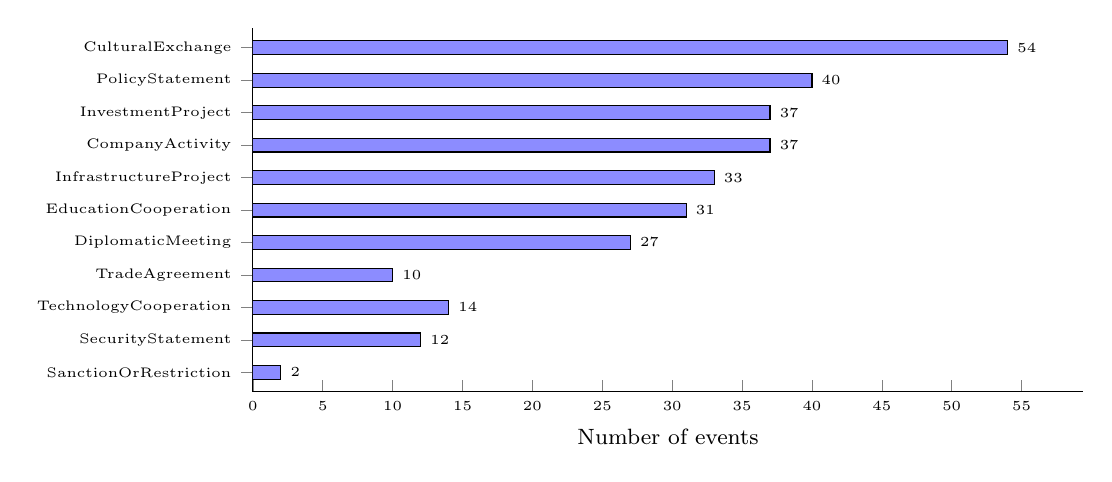
\begin{tikzpicture}
\begin{axis}[
  xbar, width=\linewidth, height=6.2cm,
  bar width=5pt,
  symbolic y coords={SanctionOrRestriction,SecurityStatement,TechnologyCooperation,
    TradeAgreement,DiplomaticMeeting,EducationCooperation,InfrastructureProject,
    CompanyActivity,InvestmentProject,PolicyStatement,CulturalExchange},
  ytick=data,
  yticklabel style={font=\tiny},
  xticklabel style={font=\tiny},
  xlabel={\footnotesize Number of events},
  xlabel style={font=\footnotesize},
  nodes near coords, nodes near coords style={font=\tiny},
  enlarge y limits=0.06,
  axis lines*=left,
  xmin=0,
]
\addplot[fill=blue!45] coordinates {
  (2,SanctionOrRestriction) (12,SecurityStatement) (14,TechnologyCooperation)
  (10,TradeAgreement) (27,DiplomaticMeeting) (31,EducationCooperation)
  (33,InfrastructureProject) (37,CompanyActivity) (37,InvestmentProject)
  (40,PolicyStatement) (54,CulturalExchange)
};
\end{axis}
\end{tikzpicture}
\caption{China--Romania bilateral events by type, full corpus ($n=297$), executed as a Cypher query against the populated Neo4j graph.}
\label{fig:timeline}
\end{figure}

\subsubsection{CQ4 -- Low-Credibility Narratives}
\textit{``Which claims later became contradicted or unverified? Which sources systematically produce low-credibility bilateral narratives?''}

Of \textbf{898} claim groups in the credibility layer's enriched output
(matching Section~\ref{sec:publisher-networks}'s publisher-network-corrected
counts; see Section~\ref{sec:cq-method} for why this, not the raw graph, is
the right source for this CQ), \textbf{851} (94.8\%) remain unresolved
(single-source), \textbf{23} are weakly supported, \textbf{16} are
contradictory, and \textbf{8} are corroborated. For contrast, the raw
graph's coarser exact-signature \texttt{Claim} grouping (no semantic merge)
yields 1{,}087 groups, 1{,}080 (99.4\%) single-source -- the semantic-merge
step alone accounts for the gap, correctly consolidating near-duplicate
reports that exact-signature matching leaves fragmented. The very high
unresolved share in both is a direct, expected consequence of the corpus's
current small scale (Section~\ref{sec:discussion}) rather than a
credibility-layer finding on its own -- most claims simply have not yet
accumulated a second independent report.

\subsubsection{CQ5 -- Collaborative Research}
\textit{``Which collaborative research has been conducted with authors from China and Romania?''}

The graph-native query surfaces \textbf{45} collaborative-research events
under the strict per-event join. A manual read still surfaces a real
precision issue worth naming rather than glossing over, at smaller scale
than the article-level approximation suggested: a share of these trace to
one long-form analytical report (a CEPA piece on Chinese influence
operations in Romania) whose prose incidentally contains trigger words
(\emph{``research,'' ``educate,'' ``collaborate''}) the rule-based
extractor matches outside any genuine collaboration-announcement context.
Genuine hits are present too (e.g.\ Green Group's Taiwan-to-Romania
technology-transfer coverage, and a minister's statement on prospective
China--Romania IT and critical-infrastructure cooperation). This remains a
real, corpus-composition-dependent limitation of trigger-lexicon event
extraction, not specific to this CQ, though the stricter per-event join
already filters out a meaningful share of the false positives the
article-level check would have kept.

\section{Implementation Details}
\label{sec:implementation}

\subsection{Technology Stack}

The system is implemented in Python~3.11. Table~\ref{tab:stack} lists
the key dependencies.

\begin{table}[htbp]
\caption{Core Technology Stack}
\label{tab:stack}
\centering
\small
\begin{tabular}{ll}
\toprule
\textbf{Component} & \textbf{Library / Tool} \\
\midrule
Article discovery    & GDELT Full-Text Search API \\
RSS ingestion        & feedparser, requests \\
Full-text extraction & trafilatura \\
Language detection   & langdetect \\
Translation          & deep-translator (Google Translate) \\
NER (rule-based)     & Python regex, custom gazetteer \\
NER (model-based)    & spaCy \texttt{en\_core\_web\_sm} \\
Relation extraction  & DeepKE (optional) \\
Temporal extraction  & py-heideltime (TIMEX3) \\
Temporal reasoning   & Allen Interval Algebra (custom) \\
Semantic matching    & sentence-transformers/all-MiniLM-L6-v2 \\
Contradiction NLI    & cross-encoder/nli-deberta-v3-xsmall \\
Intermediate storage & SQLite~3, numbered SQL migrations \\
Graph database       & Neo4j~4.x, neo4j Python driver \\
Graph visualization  & neo4j-viz, Plotly \\
Testing              & pytest (unit + integration) \\
\bottomrule
\end{tabular}
\end{table}

\subsection{Reproducibility}

All package versions are pinned in \texttt{requirements.txt}. A Conda
environment specification (\texttt{environment.yml}) allows one-command
recreation. The SQLite schema is managed via numbered migration files, so
\texttt{init\_project.py} can rebuild the database from scratch without
data loss. Neo4j indexes and constraints are applied idempotently by
\texttt{init\_graph\_schema.py}.

\subsection{Incremental Updates}

Because every article is deduplicated by URL and content hash before NLP
processing, the pipeline can safely be scheduled (e.g., daily CRON) without
re-processing previously seen articles. The GDELT fetcher accepts an
explicit \texttt{--timespan} argument (e.g., \texttt{24hours}) to restrict
the API window, minimizing redundant fetches.

% ─────────────────────────────────────────────────────────────────────────────
\section{Discussion}
\label{sec:discussion}

\paragraph{Full-text ingestion was a load-bearing fix, not a refinement}
An earlier version of the ingestion pipeline never fetched article bodies
for GDELT-sourced articles by design, assembling \texttt{content\_clean}
from title and GDELT snippet only; because GDELT's Full-Text Search API
essentially never populates a snippet, every downstream module -- entity
extraction, relation extraction, temporal extraction, and every claim in
the corroboration/credibility layer -- was in practice operating on
headline text alone. We confirmed this directly on the full ingested
corpus (every article had an empty raw-content field) before implementing
the scraping fix described in Section~\ref{sec:ingestion}. We flag this
because it changes how prior single-annotator gold-pair labeling on this
project should be read: a large fraction of real mined candidate pairs
prior to the fix were near-duplicate headline strings differing only in a
publisher's trailing site-name suffix, which is a much less discriminating
labeling task than judging genuine claim similarity over full article
content.

\paragraph{Translation at scale surfaced a silent-failure mode}
Translating short titles rarely produced enough request volume to trip the
free translation endpoint's rate limiting. Translating full article bodies
did, almost immediately, once full-text ingestion was enabled -- and, more
seriously, the client library did not always raise on failure: under
sustained rate limiting it returned the endpoint's own HTML error page text
as if it were a successful translation. We added an explicit rate-limit
delay and a defensive check that rejects responses matching the error
page's signature, treating them as translation failures rather than silently
admitting corrupted content into the corpus. We report this as a concrete
instance of a more general point: scaling up a text-processing step can
break assumptions (here, ``translation requests are infrequent enough to
never rate-limit'') that held trivially at the smaller scale the module was
originally built and tested against.

\paragraph{Multilingual coverage}
The relevance filter currently requires English-translated text for
co-mention detection. Articles in Romanian, Chinese, or other languages are
translated before filtering, which introduces latency and potential
translation artifacts. Future work could apply multilingual NER models
directly on the original text to reduce this dependency.

\paragraph{Temporal resolution}
HeidelTime performs well on absolute dates but struggles with relative
expressions whose anchor is ambiguous (e.g., ``recent weeks'' in a
republished article). The fallback regex engine mitigates this but with
lower normalization quality. Integration of the document creation time
as a DCT anchor improves relative-date resolution significantly.

\paragraph{Scalability}
SQLite provides adequate performance for the current news-stream volume
($<$10\,000 articles/month). As the corpus grows, the intermediate
store could migrate to PostgreSQL while retaining the same migration
infrastructure.

\paragraph{Lifecycle models are a first pass, not a validated ontology}
The per-event-type state machines in Section~\ref{sec:lifecycle} are
hand-authored and deliberately small (3--5 states); they have not been
validated against diplomatic- or economic-process literature, and should be
read as a framework demonstration -- the mechanism (date-ordered sequence
verification against a legal-transition graph) is the contribution, not the
specific states chosen for each of the 11 event types.

\paragraph{Annotation and evaluation scale}
The initial component ablations in Section~\ref{sec:ablations} use small
(10--12-pair), single-annotator gold sets -- sufficient to validate each
mechanism and calibrate default thresholds, not to support a strong
generalization claim on their own. Section~\ref{sec:ablations-scaled}
addresses this for two of the three components with real, much larger
mined pools (134 and 142 pairs) externally judged by independent LLM
raters, which is what surfaced the NLI contradiction detector's precision
collapse on real formulaic text -- a finding the small hand-authored set
could not have revealed. A genuine human second annotator was attempted
but not obtained this cycle (Section~\ref{sec:llm-judge} explains why and
what we substituted); the third component (contradiction-vs.-evolution)
could not be scaled with real data at all, for the data-scarcity reason
given in Section~\ref{sec:ablations-scaled}, and remains evidenced only by
its $n{=}12$ hand-authored set.

% ─────────────────────────────────────────────────────────────────────────────
\section{Conclusion}
\label{sec:conclusion}

We have presented a complete pipeline for building and incrementally
maintaining a temporal knowledge graph from a multilingual bilateral news
stream, with a focus on China--Romania relations. The system combines GDELT
article discovery with full-text extraction, curated RSS ingestion,
rule-augmented and model-based NER, HeidelTime TIMEX3 temporal
normalization, a fine-grained bilateral-relations ontology grounded in
CAMEO, GDELT, IPTC, and W3C OWL-Time, and a provenance-aware credibility
layer. Event-pair reasoning uses the complete 13-relation Allen Interval
Algebra rather than a coarse bucketed view, and the credibility layer
combines publisher-network-aware corroboration, semantic claim merging, and
NLI-based contradiction detection, gated by the Allen relations and an
explicit claim-lifecycle state machine so that ordinary claim evolution is
not mistaken for a factual contradiction. A rule-based reproduction of a
coarse time-bucket temporal representation from prior fact-checking work
serves as an ablation baseline, and the resulting comparison (Section~\ref{sec:ablations})
provides direct, if small-scale, evidence for reasoning over exact interval
relations rather than distance buckets. The Neo4j graph supports five
competency questions covering economic evolution, institutional linkages,
event enumeration, credibility assessment, and collaborative research
discovery.

The modular architecture, numbered migrations, and pinned dependencies make
the system reproducible and extensible. Future directions include
multilingual NER without translation, a validated (rather than hand-authored)
claim-lifecycle ontology grounded in domain-process literature, a larger and
multi-annotator gold evaluation set, and integration with external
fact-checking APIs for real-time contested-claim alerts.

% ─────────────────────────────────────────────────────────────────────────────
\balance
\begin{thebibliography}{00}

\bibitem{trivedi2019dyrep}
R.~Trivedi, M.~Farajtabar, P.~Biswal, and H.~Zha,
``Representation Learning over Dynamic Graphs,''
in \textit{Proc. Int. Conf. Learning Representations (ICLR)}, 2019.
[Online]. Available: \url{https://arxiv.org/abs/1803.04051}

\bibitem{gottschalk2019eventkg}
S.~Gottschalk and E.~Demidova,
``EventKG - the Hub of Event Knowledge on the Web - and Biographical Timeline Generation,''
\textit{Semantic Web Journal}, 2019.
[Online]. Available: \url{https://arxiv.org/abs/1905.08794}

\bibitem{leetaru2013gdelt}
K.~Leetaru and P.~A.~Schrodt,
``GDELT: Global database of society, language, and behavior,''
in \textit{ISA Annual Convention}, 2013.
[Online]. Available: \url{https://www.gdeltproject.org/data.html#documentation}

\bibitem{gerner2002cameo}
D.~J.~Gerner \textit{et al.},
``Conflict and Mediation Event Observations (CAMEO): A New Event Data Framework for the Analysis of Foreign Policy Interactions,''
in \textit{Annual Meeting of the International Studies Association}, 2002.
[Online]. Available: \url{https://www.researchgate.net/publication/2840364_Conflict_and_Mediation_Event_Observations_CAMEO_A_New_Event_Data_Framework_for_the_Analysis_of_Foreign_Policy_Interactions}

\bibitem{zhang2022deepke}
N.~Zhang \textit{et al.},
``DeepKE: A Deep Learning Based Knowledge Extraction Toolkit for Knowledge Base Population,''
in \textit{Proc. EMNLP (System Demonstrations)}, 2022, pp.~98--108.
[Online]. Available: \url{https://arxiv.org/abs/2201.03335}

\bibitem{strotgen2010heideltime}
J.~Str\"{o}tgen and M.~Gertz,
``HeidelTime: High Quality Rule-Based Extraction and Normalization of Temporal Expressions,''
in \textit{Proc. SemEval}, 2010, pp.~321--324.
[Online]. Available: \url{https://aclanthology.org/S10-1071/}

\bibitem{pustejovsky2003timex3}
J.~Pustejovsky \textit{et al.},
``The TIMEBANK corpus,''
in \textit{Proc. Corpus Linguistics}, 2003, pp.~647--656.
[Online]. Available: \url{https://ucrel.lancs.ac.uk/publications/CL2003/papers/pustejovsky.pdf}

\bibitem{cox2017owltime}
S.~Cox and C.~Little,
``Time ontology in OWL,'' W3C Recommendation, October 2017.
[Online]. Available: \url{https://www.w3.org/TR/owl-time/}

\bibitem{elsahar2018trex}
H.~El~Sahar \textit{et al.},
``T-REx: A Large Scale Alignment of Natural Language with Knowledge Base Triples,''
in \textit{Proc. LREC}, 2018.
[Online]. Available: \url{https://aclanthology.org/L18-1544/}

\bibitem{jain2020timeplex}
P.~Jain, S.~Rathi, Mausam, and S.~Chakrabarti,
``Temporal knowledge base completion: New algorithms and evaluation protocols,''
in \textit{Proc. EMNLP}, 2020, pp.~3733--3747.
[Online]. Available: \url{https://aclanthology.org/2020.emnlp-main.305/}

\bibitem{shu2019fakenews}
K.~Shu \textit{et al.},
``Fake news detection on social media: A data mining perspective,''
\textit{ACM SIGKDD Explorations}.
[Online]. Available: \url{https://arxiv.org/abs/1708.01967}

\bibitem{popat2018credeyecontrib}
K.~Popat \textit{et al.},
``CredEye: A Credibility Lens for Analyzing and Explaining Misinformation,''
in \textit{Proc. WWW (Companion)}, 2018.
[Online]. Available: \url{https://www.researchgate.net/publication/324630878_CredEye_A_Credibility_Lens_for_Analyzing_and_Explaining_Misinformation}

\bibitem{gruninger1995ontology}
M.~Gr\"{u}ninger and M.~S.~Fox,
``Methodology for the design and evaluation of ontologies,''
in \textit{Proc. IJCAI Workshop on Basic Ontological Issues in Knowledge Sharing}, 1995.
[Online]. Available: \url{https://www.researchgate.net/publication/2288533_Methodology_for_the_Design_and_Evaluation_of_Ontologies}

\bibitem{fader2011reverb}
A.~Fader, S.~Soderland, and O.~Etzioni,
``Identifying Relations for Open Information Extraction,''
in \textit{Proc. EMNLP}, 2011, pp.~1535--1545.
[Online]. Available: \url{https://aclanthology.org/D11-1142/}

\bibitem{allen1983interval}
J.~F.~Allen,
``Maintaining Knowledge about Temporal Intervals,''
\textit{Communications of the ACM}, vol.~26, no.~11, pp.~832--843, 1983.
[Online]. Available: \url{https://dl.acm.org/doi/10.1145/182.358434}

\bibitem{allein2023implicit}
L.~Allein, I.~Augenstein, and M.-F.~Moens,
``Implicit Temporal Reasoning for Evidence-Based Fact-Checking,''
in \textit{Findings of the Association for Computational Linguistics: EACL}, 2023.
[Online]. Available: \url{https://arxiv.org/abs/2211.09403}

\bibitem{wang2020minilm}
W.~Wang, F.~Wei, L.~Dong, H.~Bao, N.~Yang, and M.~Zhou,
``MiniLM: Deep Self-Attention Distillation for Task-Agnostic Compression of Pre-Trained Transformers,''
in \textit{Proc. NeurIPS}, 2020.
[Online]. Available: \url{https://arxiv.org/abs/2002.10957}

\bibitem{he2021debertav3}
P.~He, J.~Gao, and W.~Chen,
``DeBERTaV3: Improving DeBERTa using ELECTRA-Style Pre-Training with Gradient-Disentangled Embedding Sharing,''
\textit{arXiv preprint}, 2021.
[Online]. Available: \url{https://arxiv.org/abs/2111.09543}

\bibitem{barbaresi2021trafilatura}
A.~Barbaresi,
``Trafilatura: A Web Scraping Library and Command-Line Tool for Text Discovery and Extraction,''
in \textit{Proc. ACL-IJCNLP (System Demonstrations)}, 2021, pp.~122--131.
[Online]. Available: \url{https://aclanthology.org/2021.acl-demo.15/}

\bibitem{landiskoch1977kappa}
J.~R.~Landis and G.~G.~Koch,
``The Measurement of Observer Agreement for Categorical Data,''
\textit{Biometrics}, vol.~33, no.~1, pp.~159--174, 1977.
[Online]. Available: \url{https://www.jstor.org/stable/2529310}

\bibitem{ross2024visled}
R.~Greer, B.~Antoniussen, A.~M{\o}gelmose, and M.~Trivedi,
``Language-Driven Active Learning for Diverse Open-Set 3D Object Detection,''
\textit{arXiv preprint}, 2024.
[Online]. Available: \url{https://arxiv.org/abs/2404.12856}

\end{thebibliography}
\end{document}
